% Options for packages loaded elsewhere
\PassOptionsToPackage{unicode}{hyperref}
\PassOptionsToPackage{hyphens}{url}
%
\documentclass[
  12pt,
]{article}
\title{Exploring the Determinants of Biogas Generation Potential in
California}
\usepackage{etoolbox}
\makeatletter
\providecommand{\subtitle}[1]{% add subtitle to \maketitle
  \apptocmd{\@title}{\par {\large #1 \par}}{}{}
}
\makeatother
\subtitle{Web address for GitHub repository}
\author{Jibikeoluwa Faborode, Yinan Ding, Abhay Rao}
\date{}

\usepackage{amsmath,amssymb}
\usepackage{lmodern}
\usepackage{iftex}
\ifPDFTeX
  \usepackage[T1]{fontenc}
  \usepackage[utf8]{inputenc}
  \usepackage{textcomp} % provide euro and other symbols
\else % if luatex or xetex
  \usepackage{unicode-math}
  \defaultfontfeatures{Scale=MatchLowercase}
  \defaultfontfeatures[\rmfamily]{Ligatures=TeX,Scale=1}
  \setmainfont[]{Times New Roman}
\fi
% Use upquote if available, for straight quotes in verbatim environments
\IfFileExists{upquote.sty}{\usepackage{upquote}}{}
\IfFileExists{microtype.sty}{% use microtype if available
  \usepackage[]{microtype}
  \UseMicrotypeSet[protrusion]{basicmath} % disable protrusion for tt fonts
}{}
\makeatletter
\@ifundefined{KOMAClassName}{% if non-KOMA class
  \IfFileExists{parskip.sty}{%
    \usepackage{parskip}
  }{% else
    \setlength{\parindent}{0pt}
    \setlength{\parskip}{6pt plus 2pt minus 1pt}}
}{% if KOMA class
  \KOMAoptions{parskip=half}}
\makeatother
\usepackage{xcolor}
\IfFileExists{xurl.sty}{\usepackage{xurl}}{} % add URL line breaks if available
\IfFileExists{bookmark.sty}{\usepackage{bookmark}}{\usepackage{hyperref}}
\hypersetup{
  pdftitle={Exploring the Determinants of Biogas Generation Potential in California},
  pdfauthor={Jibikeoluwa Faborode, Yinan Ding, Abhay Rao},
  hidelinks,
  pdfcreator={LaTeX via pandoc}}
\urlstyle{same} % disable monospaced font for URLs
\usepackage[margin=2.54cm]{geometry}
\usepackage{graphicx}
\makeatletter
\def\maxwidth{\ifdim\Gin@nat@width>\linewidth\linewidth\else\Gin@nat@width\fi}
\def\maxheight{\ifdim\Gin@nat@height>\textheight\textheight\else\Gin@nat@height\fi}
\makeatother
% Scale images if necessary, so that they will not overflow the page
% margins by default, and it is still possible to overwrite the defaults
% using explicit options in \includegraphics[width, height, ...]{}
\setkeys{Gin}{width=\maxwidth,height=\maxheight,keepaspectratio}
% Set default figure placement to htbp
\makeatletter
\def\fps@figure{htbp}
\makeatother
\setlength{\emergencystretch}{3em} % prevent overfull lines
\providecommand{\tightlist}{%
  \setlength{\itemsep}{0pt}\setlength{\parskip}{0pt}}
\setcounter{secnumdepth}{5}
\ifLuaTeX
  \usepackage{selnolig}  % disable illegal ligatures
\fi

\begin{document}
\maketitle

\newpage
\tableofcontents 
\newpage
\listoftables 
\newpage

\hypertarget{table-of-figures}{%
\section{Table of figures}\label{table-of-figures}}

Figure 1: Population density across counties im California

Figure 2: Impoverished population density across counties in California

Figure 3: Total Methane potential across counties in California

Figure 4: Waste water Methane Potential across counties in California

Figure 5: Landfill methane potential across counties in California

Figure 6: Organic Waste methane potential across counties in California

Figure 7: Animal manure methane potential across counties in California

Figure 8: Total Methane Generation Potential

Figure 9:

Figure 10:

Figure 11:

Figure 12:

Figure 13:

Figure 14:

\newpage

\begin{verbatim}



\newpage

# Background

## Rationale of the study

The transition to cleaner and renewable sources of energy requires more
work to scale already existing gains, for example in the area of biogas
utilization, while also seeking out new opportunities. Biogas is a form
of renewable energy produced by anaerobic decomposition or
thermochemical conversion of biomass such as agricultural waste, manure,
municipal waste sewage, green waste and food waste. Biogas is composed
mostly of methane, alongside carbon dioxide, water vapor and other
gases. Similar to natural gas, biogas can be burned directly as a fuel
or treated to remove the CO2 and other gases before for being used in
the form of biomethane.

Utilizing biogas as an energy source helps to transform harmful gases
from decomposing waste into positive use. Methane is a powerful
greenhouse gas that traps heat in the atmosphere, with a global warming
potential estimated to be over 25 times as potent as that of Carbon
Dioxide.Transforming waste into biogas therefore reduces greenhouse gas
emissions and the risk of pollution to waterways. The
[UNECE](https://unece.org/challenge#:~:text=Methane%20is%20a%20powerful%20greenhouses,grows%20to%2084%2D86%20times.)
estimates that over a 20 year period, this ratio increases to 84-86
times. However, stored biogas limits the amount of methane released into
the atmosphere and reduces dependence on fossil fuels. When stored ,
biogas serves as a renewable and reliable baseload power source and can
even be used to rapidly meet peak power demands. When biogas is used for
energy generation in place of fossil fuels, it enables even more
emission reductions, sometimes resulting in carbon negative systems.
According to the [Environmental and Energy Study Institute,
EESI](https://www.eesi.org/papers/view/fact-sheet-biogasconverting-waste-to-energy)
,the reduction of methane emissions derived from tapping all the
potential biogas in the United States would be equal to the annual
emissions of 800,000 to 11 million passenger vehicles.

Unfortunately, despite the various benefits offered by biogas energy,
the United States currently only has 2,200 operating biogas systems. The
EESI estimates this current capacity to be less than 20% of the total
potential. It is on this basis that this study attempts to examine the
factors contributing to biogas generation potential, particularly in
California. California was selected because of its status as a leading
state in biogas generation potential based on estimates by the National
Renewable Energy Laboratory (NREL). According to the [American Biogas
Council](chrome-extension://efaidnbmnnnibpcajpcglclefindmkaj/viewer.html?pdfurl=https%3A%2F%2Famericanbiogascouncil.org%2Fwp-content%2Fuploads%2F2019%2F05%2FABCBiogasStateProfile_CA.pdf&clen=226298&chunk=true),
California can power nearly 200,000 homes if this biogas is utilized
appropriately. The results of our analysis for California can provide
the basis for further analysis across several other US states.

## Research Questions

The analysis conducted was done based on two research questions:

1.  Is biogas generation potential correlated with population density
    across California counties?

2.  What additional factors must be considered in determining biogas
    generation potential?

\newpage

# Dataset Information

the datasets used include the following:

1.  Methane Generation Potential The NREL's dataset on methane
    generation potential covers data for the entire United States of
    America. It particularly providing information for Methane
    generation potential across all states in metric tons from sources
    which include landfills, industrial organic waste, animal manure,
    and wastewater . All of these individual sources were aggregated to
    estimate total methane generation potential by state. The dataset
    contained estimates for 2009 to 2012, being the latest available
    data we could find online.

2.  Population data Population data was pulled from the latest available
    the Social Vulnerability Index data compiled by the Center for
    Disease Control (CDC) and Agency for Toxic Substance and Diseace
    Reegistry (ATSDR). This dataset also includes details on
    impoverished populations and spans from 2017-2018. Since the SDI
    offers data that helps to effectly plan towards meeting the needs of
    improverished populations, this dataset also helps to dds another
    dimension to our analysis as it enables the exploration of impacts
    on socially vulnerable people.

\newpage

# Exploratory Analysis

The two datasets were wrangled and joined both datasets to have a
unified dataframe that captured data on methane generation potential,
population and poverty levels by county. An initial exploration of the
data was done to provide a visual assessment of spatial data and
determine the emergence of any any trends.



\end{verbatim}

\hypertarget{simple-feature-collection-with-6-features-and-14-fields}{%
\subsection{Simple feature collection with 6 features and 14
fields}\label{simple-feature-collection-with-6-features-and-14-fields}}

\hypertarget{geometry-type-multipolygon}{%
\subsection{Geometry type:
MULTIPOLYGON}\label{geometry-type-multipolygon}}

\hypertarget{dimension-xy}{%
\subsection{Dimension: XY}\label{dimension-xy}}

\hypertarget{bounding-box-xmin--122.7851-ymin-37.45447-xmax--119.5423-ymax-40.15203}{%
\subsection{Bounding box: xmin: -122.7851 ymin: 37.45447 xmax: -119.5423
ymax:
40.15203}\label{bounding-box-xmin--122.7851-ymin-37.45447-xmax--119.5423-ymax-40.15203}}

\hypertarget{geodetic-crs-wgs-84}{%
\subsection{Geodetic CRS: WGS 84}\label{geodetic-crs-wgs-84}}

\hypertarget{objectid-name-state_name-fips-owch4t-amch4t-wwtpch4t}{%
\subsection{ObjectID NAME STATE\_NAME FIPS OWCH4t AMCH4t
WWTPCH4t}\label{objectid-name-state_name-fips-owch4t-amch4t-wwtpch4t}}

\hypertarget{alameda-california-06001-5700.695190-0.367359-10461.687700}{%
\subsection{1 184 Alameda California 06001 5700.695190 0.367359
10461.687700}\label{alameda-california-06001-5700.695190-0.367359-10461.687700}}

\hypertarget{alpine-california-06003-6.483819-0.000000-6.667176}{%
\subsection{2 185 Alpine California 06003 6.483819 0.000000
6.667176}\label{alpine-california-06003-6.483819-0.000000-6.667176}}

\hypertarget{amador-california-06005-156.310667-3.826180-624.136548}{%
\subsection{3 186 Amador California 06005 156.310667 3.826180
624.136548}\label{amador-california-06005-156.310667-3.826180-624.136548}}

\hypertarget{butte-california-06007-817.909133-20.460013-1210.759120}{%
\subsection{4 187 Butte California 06007 817.909133 20.460013
1210.759120}\label{butte-california-06007-817.909133-20.460013-1210.759120}}

\hypertarget{calaveras-california-06009-97.664105-11.663426-200.148617}{%
\subsection{5 188 Calaveras California 06009 97.664105 11.663426
200.148617}\label{calaveras-california-06009-97.664105-11.663426-200.148617}}

\hypertarget{colusa-california-06011-72.199705-2.057210-104.007942}{%
\subsection{6 189 Colusa California 06011 72.199705 2.057210
104.007942}\label{colusa-california-06011-72.199705-2.057210-104.007942}}

\hypertarget{lfgch4t-totalch4t-county-location-e_totpop-e_pov}{%
\subsection{LFGCH4t TotalCH4t COUNTY LOCATION E\_TOTPOP
E\_POV}\label{lfgch4t-totalch4t-county-location-e_totpop-e_pov}}

\hypertarget{alameda-alameda-county-california-1643700-170884}{%
\subsection{1 49311 65473.75020 Alameda Alameda County, California
1643700 170884}\label{alameda-alameda-county-california-1643700-170884}}

\hypertarget{alpine-alpine-county-california-1146-227}{%
\subsection{2 0 13.15099 Alpine Alpine County, California 1146
227}\label{alpine-alpine-county-california-1146-227}}

\hypertarget{amador-amador-county-california-37829-3323}{%
\subsection{3 0 784.27340 Amador Amador County, California 37829
3323}\label{amador-amador-county-california-37829-3323}}

\hypertarget{butte-butte-county-california-227075-44410}{%
\subsection{4 0 2049.12827 Butte Butte County, California 227075
44410}\label{butte-butte-county-california-227075-44410}}

\hypertarget{calaveras-calaveras-county-california-45235-5242}{%
\subsection{5 0 309.47615 Calaveras Calaveras County, California 45235
5242}\label{calaveras-calaveras-county-california-45235-5242}}

\hypertarget{colusa-colusa-county-california-21464-2929}{%
\subsection{6 0 178.26486 Colusa Colusa County, California 21464
2929}\label{colusa-colusa-county-california-21464-2929}}

\hypertarget{e_minrty-geometry}{%
\subsection{E\_MINRTY geometry}\label{e_minrty-geometry}}

\hypertarget{multipolygon--122.313-37}{%
\subsection{1 1120309 MULTIPOLYGON (((-122.313
37\ldots{}}\label{multipolygon--122.313-37}}

\hypertarget{multipolygon--120.0726-3}{%
\subsection{2 468 MULTIPOLYGON (((-120.0726
3\ldots{}}\label{multipolygon--120.0726-3}}

\hypertarget{multipolygon--121.0276-3}{%
\subsection{3 8066 MULTIPOLYGON (((-121.0276
3\ldots{}}\label{multipolygon--121.0276-3}}

\hypertarget{multipolygon--122.0573-3}{%
\subsection{4 62685 MULTIPOLYGON (((-122.0573
3\ldots{}}\label{multipolygon--122.0573-3}}

\hypertarget{multipolygon--120.9955-3}{%
\subsection{5 8330 MULTIPOLYGON (((-120.9955
3\ldots{}}\label{multipolygon--120.9955-3}}

\hypertarget{multipolygon--122.7851-3}{%
\subsection{6 13792 MULTIPOLYGON (((-122.7851
3\ldots{}}\label{multipolygon--122.7851-3}}

\begin{verbatim}
Visually, the most populated area of California, given by the county
shaded yellow, Los Angeles, has the highest methane (CH4) generation
potential. The density of impoverished population appears to be
similarly distributed.

![](FDR_Final_files/figure-latex/unnamed-chunk-3-1.pdf)<!-- --> 

The total Methane generation potential is greatest at the most densely
populated areas. This trend appears to continue with wastewater derived
methane.

![](FDR_Final_files/figure-latex/unnamed-chunk-4-1.pdf)<!-- --> 

Industrial Organic waste, like wastewater, is highly correlated with
population.With landfill-based methane, some counties in central CA,
which do not appear to have a high population, have comparatively high
methane generation potential. There may be some non-population related
factors in play.

![](FDR_Final_files/figure-latex/unnamed-chunk-5-1.pdf)<!-- --> 

The trend with animal-manure derived CH4 however substantially differs
from the previous cases. Population does not appear to be a decisive
factor.

![](FDR_Final_files/figure-latex/unnamed-chunk-6-1.pdf)<!-- --> 

\newpage

# Analysis

## Question 1: What factors affect biogas generation potential in different counties of California? Could it have potential correlations with the population size?

\end{verbatim}

\hypertarget{section}{%
\subsection{}\label{section}}

\hypertarget{pearsons-product-moment-correlation}{%
\subsection{Pearson's product-moment
correlation}\label{pearsons-product-moment-correlation}}

\hypertarget{section-1}{%
\subsection{}\label{section-1}}

\hypertarget{data-svi_sf_jointotalch4t-and-svi_sf_joine_totpop}{%
\subsection{\texorpdfstring{data:
svi\_sf\_join\(TotalCH4t and svi_sf_join\)E\_TOTPOP}{data: svi\_sf\_joinTotalCH4t and svi\_sf\_joinE\_TOTPOP}}\label{data-svi_sf_jointotalch4t-and-svi_sf_joine_totpop}}

\hypertarget{t-10.655-df-56-p-value-4.365e-15}{%
\subsection{t = 10.655, df = 56, p-value =
4.365e-15}\label{t-10.655-df-56-p-value-4.365e-15}}

\hypertarget{alternative-hypothesis-true-correlation-is-not-equal-to-0}{%
\subsection{alternative hypothesis: true correlation is not equal to
0}\label{alternative-hypothesis-true-correlation-is-not-equal-to-0}}

\hypertarget{percent-confidence-interval}{%
\subsection{95 percent confidence
interval:}\label{percent-confidence-interval}}

\hypertarget{section-2}{%
\subsection{0.7101412 0.8887681}\label{section-2}}

\hypertarget{sample-estimates}{%
\subsection{sample estimates:}\label{sample-estimates}}

\hypertarget{cor}{%
\subsection{cor}\label{cor}}

\hypertarget{section-3}{%
\subsection{0.818333}\label{section-3}}

\begin{verbatim}
\end{verbatim}

\hypertarget{section-4}{%
\subsection{}\label{section-4}}

\hypertarget{call}{%
\subsection{Call:}\label{call}}

\hypertarget{lmformula-svi_sf_jointotalch4t-svi_sf_joine_totpop}{%
\subsection{\texorpdfstring{lm(formula =
svi\_sf\_join\(TotalCH4t ~ svi_sf_join\)E\_TOTPOP)}{lm(formula = svi\_sf\_joinTotalCH4t \textasciitilde{} svi\_sf\_joinE\_TOTPOP)}}\label{lmformula-svi_sf_jointotalch4t-svi_sf_joine_totpop}}

\hypertarget{section-5}{%
\subsection{}\label{section-5}}

\hypertarget{residuals}{%
\subsection{Residuals:}\label{residuals}}

\hypertarget{min-1q-median-3q-max}{%
\subsection{Min 1Q Median 3Q Max}\label{min-1q-median-3q-max}}

\hypertarget{section-6}{%
\subsection{-34706 -8182 -6090 -3565 76153}\label{section-6}}

\hypertarget{section-7}{%
\subsection{}\label{section-7}}

\hypertarget{coefficients}{%
\subsection{Coefficients:}\label{coefficients}}

\hypertarget{estimate-std.-error-t-value-prt}{%
\subsection{Estimate Std. Error t value
Pr(\textgreater\textbar t\textbar)}\label{estimate-std.-error-t-value-prt}}

\hypertarget{intercept-5.836e03-2.956e03-1.974-0.0533-.}{%
\subsection{(Intercept) 5.836e+03 2.956e+03 1.974 0.0533
.}\label{intercept-5.836e03-2.956e03-1.974-0.0533-.}}

\hypertarget{svi_sf_joine_totpop-1.962e-02-1.841e-03-10.655-4.36e-15}{%
\subsection{svi\_sf\_join\$E\_TOTPOP 1.962e-02 1.841e-03 10.655 4.36e-15
***}\label{svi_sf_joine_totpop-1.962e-02-1.841e-03-10.655-4.36e-15}}

\hypertarget{section-8}{%
\subsection{---}\label{section-8}}

\hypertarget{signif.-codes-0-0.001-0.01-0.05-.-0.1-1}{%
\subsection{\texorpdfstring{Signif. codes: 0 `\emph{\textbf{' 0.001 '}'
0.01 '}' 0.05 `.' 0.1 ' '
1}{Signif. codes: 0 `\,' 0.001 '\,' 0.01 '\,' 0.05 `.' 0.1 ' ' 1}}\label{signif.-codes-0-0.001-0.01-0.05-.-0.1-1}}

\hypertarget{section-9}{%
\subsection{}\label{section-9}}

\hypertarget{residual-standard-error-20430-on-56-degrees-of-freedom}{%
\subsection{Residual standard error: 20430 on 56 degrees of
freedom}\label{residual-standard-error-20430-on-56-degrees-of-freedom}}

\hypertarget{multiple-r-squared-0.6697-adjusted-r-squared-0.6638}{%
\subsection{Multiple R-squared: 0.6697, Adjusted R-squared:
0.6638}\label{multiple-r-squared-0.6697-adjusted-r-squared-0.6638}}

\hypertarget{f-statistic-113.5-on-1-and-56-df-p-value-4.365e-15}{%
\subsection{F-statistic: 113.5 on 1 and 56 DF, p-value:
4.365e-15}\label{f-statistic-113.5-on-1-and-56-df-p-value-4.365e-15}}

\begin{verbatim}
![](FDR_Final_files/figure-latex/unnamed-chunk-7-1.pdf)<!-- --> ![](FDR_Final_files/figure-latex/unnamed-chunk-7-2.pdf)<!-- --> ![](FDR_Final_files/figure-latex/unnamed-chunk-7-3.pdf)<!-- --> ![](FDR_Final_files/figure-latex/unnamed-chunk-7-4.pdf)<!-- --> ![](FDR_Final_files/figure-latex/unnamed-chunk-7-5.pdf)<!-- --> 
\end{verbatim}

\hypertarget{section-10}{%
\subsection{}\label{section-10}}

\hypertarget{pearsons-product-moment-correlation-1}{%
\subsection{Pearson's product-moment
correlation}\label{pearsons-product-moment-correlation-1}}

\hypertarget{section-11}{%
\subsection{}\label{section-11}}

\hypertarget{data-svi_sf_joinowch4t-and-svi_sf_joine_totpop}{%
\subsection{\texorpdfstring{data:
svi\_sf\_join\(OWCH4t and svi_sf_join\)E\_TOTPOP}{data: svi\_sf\_joinOWCH4t and svi\_sf\_joinE\_TOTPOP}}\label{data-svi_sf_joinowch4t-and-svi_sf_joine_totpop}}

\hypertarget{t-82.353-df-56-p-value-2.2e-16}{%
\subsection{t = 82.353, df = 56, p-value \textless{}
2.2e-16}\label{t-82.353-df-56-p-value-2.2e-16}}

\hypertarget{alternative-hypothesis-true-correlation-is-not-equal-to-0-1}{%
\subsection{alternative hypothesis: true correlation is not equal to
0}\label{alternative-hypothesis-true-correlation-is-not-equal-to-0-1}}

\hypertarget{percent-confidence-interval-1}{%
\subsection{95 percent confidence
interval:}\label{percent-confidence-interval-1}}

\hypertarget{section-12}{%
\subsection{0.9930490 0.9975794}\label{section-12}}

\hypertarget{sample-estimates-1}{%
\subsection{sample estimates:}\label{sample-estimates-1}}

\hypertarget{cor-1}{%
\subsection{cor}\label{cor-1}}

\hypertarget{section-13}{%
\subsection{0.9958969}\label{section-13}}

\begin{verbatim}
\end{verbatim}

\hypertarget{section-14}{%
\subsection{}\label{section-14}}

\hypertarget{call-1}{%
\subsection{Call:}\label{call-1}}

\hypertarget{lmformula-svi_sf_joinowch4t-svi_sf_joine_totpop}{%
\subsection{\texorpdfstring{lm(formula =
svi\_sf\_join\(OWCH4t ~ svi_sf_join\)E\_TOTPOP)}{lm(formula = svi\_sf\_joinOWCH4t \textasciitilde{} svi\_sf\_joinE\_TOTPOP)}}\label{lmformula-svi_sf_joinowch4t-svi_sf_joine_totpop}}

\hypertarget{section-15}{%
\subsection{}\label{section-15}}

\hypertarget{residuals-1}{%
\subsection{Residuals:}\label{residuals-1}}

\hypertarget{min-1q-median-3q-max-1}{%
\subsection{Min 1Q Median 3Q Max}\label{min-1q-median-3q-max-1}}

\hypertarget{section-16}{%
\subsection{-1801.49 -77.14 28.39 100.93 1809.74}\label{section-16}}

\hypertarget{section-17}{%
\subsection{}\label{section-17}}

\hypertarget{coefficients-1}{%
\subsection{Coefficients:}\label{coefficients-1}}

\hypertarget{estimate-std.-error-t-value-prt-1}{%
\subsection{Estimate Std. Error t value
Pr(\textgreater\textbar t\textbar)}\label{estimate-std.-error-t-value-prt-1}}

\hypertarget{intercept--4.289e01-7.117e01--0.603-0.549}{%
\subsection{(Intercept) -4.289e+01 7.117e+01 -0.603
0.549}\label{intercept--4.289e01-7.117e01--0.603-0.549}}

\hypertarget{svi_sf_joine_totpop-3.650e-03-4.432e-05-82.353-2e-16}{%
\subsection{svi\_sf\_join\$E\_TOTPOP 3.650e-03 4.432e-05 82.353
\textless2e-16
***}\label{svi_sf_joine_totpop-3.650e-03-4.432e-05-82.353-2e-16}}

\hypertarget{section-18}{%
\subsection{---}\label{section-18}}

\hypertarget{signif.-codes-0-0.001-0.01-0.05-.-0.1-1-1}{%
\subsection{\texorpdfstring{Signif. codes: 0 `\emph{\textbf{' 0.001 '}'
0.01 '}' 0.05 `.' 0.1 ' '
1}{Signif. codes: 0 `\,' 0.001 '\,' 0.01 '\,' 0.05 `.' 0.1 ' ' 1}}\label{signif.-codes-0-0.001-0.01-0.05-.-0.1-1-1}}

\hypertarget{section-19}{%
\subsection{}\label{section-19}}

\hypertarget{residual-standard-error-491.8-on-56-degrees-of-freedom}{%
\subsection{Residual standard error: 491.8 on 56 degrees of
freedom}\label{residual-standard-error-491.8-on-56-degrees-of-freedom}}

\hypertarget{multiple-r-squared-0.9918-adjusted-r-squared-0.9917}{%
\subsection{Multiple R-squared: 0.9918, Adjusted R-squared:
0.9917}\label{multiple-r-squared-0.9918-adjusted-r-squared-0.9917}}

\hypertarget{f-statistic-6782-on-1-and-56-df-p-value-2.2e-16}{%
\subsection{F-statistic: 6782 on 1 and 56 DF, p-value: \textless{}
2.2e-16}\label{f-statistic-6782-on-1-and-56-df-p-value-2.2e-16}}

\begin{verbatim}
\end{verbatim}

\hypertarget{section-20}{%
\subsection{}\label{section-20}}

\hypertarget{pearsons-product-moment-correlation-2}{%
\subsection{Pearson's product-moment
correlation}\label{pearsons-product-moment-correlation-2}}

\hypertarget{section-21}{%
\subsection{}\label{section-21}}

\hypertarget{data-svi_sf_joinamch4t-and-svi_sf_joine_totpop}{%
\subsection{\texorpdfstring{data:
svi\_sf\_join\(AMCH4t and svi_sf_join\)E\_TOTPOP}{data: svi\_sf\_joinAMCH4t and svi\_sf\_joinE\_TOTPOP}}\label{data-svi_sf_joinamch4t-and-svi_sf_joine_totpop}}

\hypertarget{t--0.02427-df-56-p-value-0.9807}{%
\subsection{t = -0.02427, df = 56, p-value =
0.9807}\label{t--0.02427-df-56-p-value-0.9807}}

\hypertarget{alternative-hypothesis-true-correlation-is-not-equal-to-0-2}{%
\subsection{alternative hypothesis: true correlation is not equal to
0}\label{alternative-hypothesis-true-correlation-is-not-equal-to-0-2}}

\hypertarget{percent-confidence-interval-2}{%
\subsection{95 percent confidence
interval:}\label{percent-confidence-interval-2}}

\hypertarget{section-22}{%
\subsection{-0.2613200 0.2552665}\label{section-22}}

\hypertarget{sample-estimates-2}{%
\subsection{sample estimates:}\label{sample-estimates-2}}

\hypertarget{cor-2}{%
\subsection{cor}\label{cor-2}}

\hypertarget{section-23}{%
\subsection{-0.003243157}\label{section-23}}

\begin{verbatim}
\end{verbatim}

\hypertarget{section-24}{%
\subsection{}\label{section-24}}

\hypertarget{call-2}{%
\subsection{Call:}\label{call-2}}

\hypertarget{lmformula-svi_sf_joinamch4t-svi_sf_joine_totpop}{%
\subsection{\texorpdfstring{lm(formula =
svi\_sf\_join\(AMCH4t ~ svi_sf_join\)E\_TOTPOP)}{lm(formula = svi\_sf\_joinAMCH4t \textasciitilde{} svi\_sf\_joinE\_TOTPOP)}}\label{lmformula-svi_sf_joinamch4t-svi_sf_joine_totpop}}

\hypertarget{section-25}{%
\subsection{}\label{section-25}}

\hypertarget{residuals-2}{%
\subsection{Residuals:}\label{residuals-2}}

\hypertarget{min-1q-median-3q-max-2}{%
\subsection{Min 1Q Median 3Q Max}\label{min-1q-median-3q-max-2}}

\hypertarget{section-26}{%
\subsection{-5569 -5558 -5523 -3877 76775}\label{section-26}}

\hypertarget{section-27}{%
\subsection{}\label{section-27}}

\hypertarget{coefficients-2}{%
\subsection{Coefficients:}\label{coefficients-2}}

\hypertarget{estimate-std.-error-t-value-prt-2}{%
\subsection{Estimate Std. Error t value
Pr(\textgreater\textbar t\textbar)}\label{estimate-std.-error-t-value-prt-2}}

\hypertarget{intercept-5.569e03-2.053e03-2.712-0.00885}{%
\subsection{(Intercept) 5.569e+03 2.053e+03 2.712 0.00885
**}\label{intercept-5.569e03-2.053e03-2.712-0.00885}}

\hypertarget{svi_sf_joine_totpop--3.103e-05-1.279e-03--0.024-0.98072}{%
\subsection{svi\_sf\_join\$E\_TOTPOP -3.103e-05 1.279e-03 -0.024
0.98072}\label{svi_sf_joine_totpop--3.103e-05-1.279e-03--0.024-0.98072}}

\hypertarget{section-28}{%
\subsection{---}\label{section-28}}

\hypertarget{signif.-codes-0-0.001-0.01-0.05-.-0.1-1-2}{%
\subsection{\texorpdfstring{Signif. codes: 0 `\emph{\textbf{' 0.001 '}'
0.01 '}' 0.05 `.' 0.1 ' '
1}{Signif. codes: 0 `\,' 0.001 '\,' 0.01 '\,' 0.05 `.' 0.1 ' ' 1}}\label{signif.-codes-0-0.001-0.01-0.05-.-0.1-1-2}}

\hypertarget{section-29}{%
\subsection{}\label{section-29}}

\hypertarget{residual-standard-error-14190-on-56-degrees-of-freedom}{%
\subsection{Residual standard error: 14190 on 56 degrees of
freedom}\label{residual-standard-error-14190-on-56-degrees-of-freedom}}

\hypertarget{multiple-r-squared-1.052e-05-adjusted-r-squared--0.01785}{%
\subsection{Multiple R-squared: 1.052e-05, Adjusted R-squared:
-0.01785}\label{multiple-r-squared-1.052e-05-adjusted-r-squared--0.01785}}

\hypertarget{f-statistic-0.000589-on-1-and-56-df-p-value-0.9807}{%
\subsection{F-statistic: 0.000589 on 1 and 56 DF, p-value:
0.9807}\label{f-statistic-0.000589-on-1-and-56-df-p-value-0.9807}}

\begin{verbatim}
\end{verbatim}

\hypertarget{section-30}{%
\subsection{}\label{section-30}}

\hypertarget{pearsons-product-moment-correlation-3}{%
\subsection{Pearson's product-moment
correlation}\label{pearsons-product-moment-correlation-3}}

\hypertarget{section-31}{%
\subsection{}\label{section-31}}

\hypertarget{data-svi_sf_joinwwtpch4t-and-svi_sf_joine_totpop}{%
\subsection{\texorpdfstring{data:
svi\_sf\_join\(WWTPCH4t and svi_sf_join\)E\_TOTPOP}{data: svi\_sf\_joinWWTPCH4t and svi\_sf\_joinE\_TOTPOP}}\label{data-svi_sf_joinwwtpch4t-and-svi_sf_joine_totpop}}

\hypertarget{t-57.684-df-56-p-value-2.2e-16}{%
\subsection{t = 57.684, df = 56, p-value \textless{}
2.2e-16}\label{t-57.684-df-56-p-value-2.2e-16}}

\hypertarget{alternative-hypothesis-true-correlation-is-not-equal-to-0-3}{%
\subsection{alternative hypothesis: true correlation is not equal to
0}\label{alternative-hypothesis-true-correlation-is-not-equal-to-0-3}}

\hypertarget{percent-confidence-interval-3}{%
\subsection{95 percent confidence
interval:}\label{percent-confidence-interval-3}}

\hypertarget{section-32}{%
\subsection{0.9859425 0.9950932}\label{section-32}}

\hypertarget{sample-estimates-3}{%
\subsection{sample estimates:}\label{sample-estimates-3}}

\hypertarget{cor-3}{%
\subsection{cor}\label{cor-3}}

\hypertarget{section-33}{%
\subsection{0.9916898}\label{section-33}}

\begin{verbatim}
\end{verbatim}

\hypertarget{section-34}{%
\subsection{}\label{section-34}}

\hypertarget{call-3}{%
\subsection{Call:}\label{call-3}}

\hypertarget{lmformula-svi_sf_joinwwtpch4t-svi_sf_joine_totpop}{%
\subsection{\texorpdfstring{lm(formula =
svi\_sf\_join\(WWTPCH4t ~ svi_sf_join\)E\_TOTPOP)}{lm(formula = svi\_sf\_joinWWTPCH4t \textasciitilde{} svi\_sf\_joinE\_TOTPOP)}}\label{lmformula-svi_sf_joinwwtpch4t-svi_sf_joine_totpop}}

\hypertarget{section-35}{%
\subsection{}\label{section-35}}

\hypertarget{residuals-3}{%
\subsection{Residuals:}\label{residuals-3}}

\hypertarget{min-1q-median-3q-max-3}{%
\subsection{Min 1Q Median 3Q Max}\label{min-1q-median-3q-max-3}}

\hypertarget{section-36}{%
\subsection{-6663.5 -147.9 65.7 168.0 3785.4}\label{section-36}}

\hypertarget{section-37}{%
\subsection{}\label{section-37}}

\hypertarget{coefficients-3}{%
\subsection{Coefficients:}\label{coefficients-3}}

\hypertarget{estimate-std.-error-t-value-prt-3}{%
\subsection{Estimate Std. Error t value
Pr(\textgreater\textbar t\textbar)}\label{estimate-std.-error-t-value-prt-3}}

\hypertarget{intercept--1.466e02-1.637e02--0.895-0.375}{%
\subsection{(Intercept) -1.466e+02 1.637e+02 -0.895
0.375}\label{intercept--1.466e02-1.637e02--0.895-0.375}}

\hypertarget{svi_sf_joine_totpop-5.882e-03-1.020e-04-57.684-2e-16}{%
\subsection{svi\_sf\_join\$E\_TOTPOP 5.882e-03 1.020e-04 57.684
\textless2e-16
***}\label{svi_sf_joine_totpop-5.882e-03-1.020e-04-57.684-2e-16}}

\hypertarget{section-38}{%
\subsection{---}\label{section-38}}

\hypertarget{signif.-codes-0-0.001-0.01-0.05-.-0.1-1-3}{%
\subsection{\texorpdfstring{Signif. codes: 0 `\emph{\textbf{' 0.001 '}'
0.01 '}' 0.05 `.' 0.1 ' '
1}{Signif. codes: 0 `\,' 0.001 '\,' 0.01 '\,' 0.05 `.' 0.1 ' ' 1}}\label{signif.-codes-0-0.001-0.01-0.05-.-0.1-1-3}}

\hypertarget{section-39}{%
\subsection{}\label{section-39}}

\hypertarget{residual-standard-error-1131-on-56-degrees-of-freedom}{%
\subsection{Residual standard error: 1131 on 56 degrees of
freedom}\label{residual-standard-error-1131-on-56-degrees-of-freedom}}

\hypertarget{multiple-r-squared-0.9834-adjusted-r-squared-0.9832}{%
\subsection{Multiple R-squared: 0.9834, Adjusted R-squared:
0.9832}\label{multiple-r-squared-0.9834-adjusted-r-squared-0.9832}}

\hypertarget{f-statistic-3327-on-1-and-56-df-p-value-2.2e-16}{%
\subsection{F-statistic: 3327 on 1 and 56 DF, p-value: \textless{}
2.2e-16}\label{f-statistic-3327-on-1-and-56-df-p-value-2.2e-16}}

\begin{verbatim}
\end{verbatim}

\hypertarget{section-40}{%
\subsection{}\label{section-40}}

\hypertarget{pearsons-product-moment-correlation-4}{%
\subsection{Pearson's product-moment
correlation}\label{pearsons-product-moment-correlation-4}}

\hypertarget{section-41}{%
\subsection{}\label{section-41}}

\hypertarget{data-svi_sf_joinlfgch4t-and-svi_sf_joine_totpop}{%
\subsection{\texorpdfstring{data:
svi\_sf\_join\(LFGCH4t and svi_sf_join\)E\_TOTPOP}{data: svi\_sf\_joinLFGCH4t and svi\_sf\_joinE\_TOTPOP}}\label{data-svi_sf_joinlfgch4t-and-svi_sf_joine_totpop}}

\hypertarget{t-9.6217-df-56-p-value-1.815e-13}{%
\subsection{t = 9.6217, df = 56, p-value =
1.815e-13}\label{t-9.6217-df-56-p-value-1.815e-13}}

\hypertarget{alternative-hypothesis-true-correlation-is-not-equal-to-0-4}{%
\subsection{alternative hypothesis: true correlation is not equal to
0}\label{alternative-hypothesis-true-correlation-is-not-equal-to-0-4}}

\hypertarget{percent-confidence-interval-4}{%
\subsection{95 percent confidence
interval:}\label{percent-confidence-interval-4}}

\hypertarget{section-42}{%
\subsection{0.6670743 0.8702275}\label{section-42}}

\hypertarget{sample-estimates-4}{%
\subsection{sample estimates:}\label{sample-estimates-4}}

\hypertarget{cor-4}{%
\subsection{cor}\label{cor-4}}

\hypertarget{section-43}{%
\subsection{0.7893612}\label{section-43}}

\begin{verbatim}
\end{verbatim}

\hypertarget{section-44}{%
\subsection{}\label{section-44}}

\hypertarget{call-4}{%
\subsection{Call:}\label{call-4}}

\hypertarget{lmformula-svi_sf_joinlfgch4t-svi_sf_joine_totpop}{%
\subsection{\texorpdfstring{lm(formula =
svi\_sf\_join\(LFGCH4t ~ svi_sf_join\)E\_TOTPOP)}{lm(formula = svi\_sf\_joinLFGCH4t \textasciitilde{} svi\_sf\_joinE\_TOTPOP)}}\label{lmformula-svi_sf_joinlfgch4t-svi_sf_joine_totpop}}

\hypertarget{section-45}{%
\subsection{}\label{section-45}}

\hypertarget{residuals-4}{%
\subsection{Residuals:}\label{residuals-4}}

\hypertarget{min-1q-median-3q-max-4}{%
\subsection{Min 1Q Median 3Q Max}\label{min-1q-median-3q-max-4}}

\hypertarget{section-46}{%
\subsection{-31207 -3285 -1030 -501 46121}\label{section-46}}

\hypertarget{section-47}{%
\subsection{}\label{section-47}}

\hypertarget{coefficients-4}{%
\subsection{Coefficients:}\label{coefficients-4}}

\hypertarget{estimate-std.-error-t-value-prt-4}{%
\subsection{Estimate Std. Error t value
Pr(\textgreater\textbar t\textbar)}\label{estimate-std.-error-t-value-prt-4}}

\hypertarget{intercept-4.564e02-1.688e03-0.270-0.788}{%
\subsection{(Intercept) 4.564e+02 1.688e+03 0.270
0.788}\label{intercept-4.564e02-1.688e03-0.270-0.788}}

\hypertarget{svi_sf_joine_totpop-1.012e-02-1.052e-03-9.622-1.81e-13}{%
\subsection{svi\_sf\_join\$E\_TOTPOP 1.012e-02 1.052e-03 9.622 1.81e-13
***}\label{svi_sf_joine_totpop-1.012e-02-1.052e-03-9.622-1.81e-13}}

\hypertarget{section-48}{%
\subsection{---}\label{section-48}}

\hypertarget{signif.-codes-0-0.001-0.01-0.05-.-0.1-1-4}{%
\subsection{\texorpdfstring{Signif. codes: 0 `\emph{\textbf{' 0.001 '}'
0.01 '}' 0.05 `.' 0.1 ' '
1}{Signif. codes: 0 `\,' 0.001 '\,' 0.01 '\,' 0.05 `.' 0.1 ' ' 1}}\label{signif.-codes-0-0.001-0.01-0.05-.-0.1-1-4}}

\hypertarget{section-49}{%
\subsection{}\label{section-49}}

\hypertarget{residual-standard-error-11670-on-56-degrees-of-freedom}{%
\subsection{Residual standard error: 11670 on 56 degrees of
freedom}\label{residual-standard-error-11670-on-56-degrees-of-freedom}}

\hypertarget{multiple-r-squared-0.6231-adjusted-r-squared-0.6164}{%
\subsection{Multiple R-squared: 0.6231, Adjusted R-squared:
0.6164}\label{multiple-r-squared-0.6231-adjusted-r-squared-0.6164}}

\hypertarget{f-statistic-92.58-on-1-and-56-df-p-value-1.815e-13}{%
\subsection{F-statistic: 92.58 on 1 and 56 DF, p-value:
1.815e-13}\label{f-statistic-92.58-on-1-and-56-df-p-value-1.815e-13}}

\begin{verbatim}
![](FDR_Final_files/figure-latex/unnamed-chunk-7-6.pdf)<!-- --> 
\end{verbatim}

\hypertarget{section-50}{%
\subsection{}\label{section-50}}

\hypertarget{pearsons-product-moment-correlation-5}{%
\subsection{Pearson's product-moment
correlation}\label{pearsons-product-moment-correlation-5}}

\hypertarget{section-51}{%
\subsection{}\label{section-51}}

\hypertarget{data-svi_sf_jointotalch4t-and-svi_sf_joine_pov}{%
\subsection{\texorpdfstring{data:
svi\_sf\_join\(TotalCH4t and svi_sf_join\)E\_POV}{data: svi\_sf\_joinTotalCH4t and svi\_sf\_joinE\_POV}}\label{data-svi_sf_jointotalch4t-and-svi_sf_joine_pov}}

\hypertarget{t-11.12-df-56-p-value-8.476e-16}{%
\subsection{t = 11.12, df = 56, p-value =
8.476e-16}\label{t-11.12-df-56-p-value-8.476e-16}}

\hypertarget{alternative-hypothesis-true-correlation-is-not-equal-to-0-5}{%
\subsection{alternative hypothesis: true correlation is not equal to
0}\label{alternative-hypothesis-true-correlation-is-not-equal-to-0-5}}

\hypertarget{percent-confidence-interval-5}{%
\subsection{95 percent confidence
interval:}\label{percent-confidence-interval-5}}

\hypertarget{section-52}{%
\subsection{0.7271725 0.8959424}\label{section-52}}

\hypertarget{sample-estimates-5}{%
\subsection{sample estimates:}\label{sample-estimates-5}}

\hypertarget{cor-5}{%
\subsection{cor}\label{cor-5}}

\hypertarget{section-53}{%
\subsection{0.8296405}\label{section-53}}

\begin{verbatim}
\end{verbatim}

\hypertarget{section-54}{%
\subsection{}\label{section-54}}

\hypertarget{call-5}{%
\subsection{Call:}\label{call-5}}

\hypertarget{lmformula-svi_sf_jointotalch4t-svi_sf_joine_pov}{%
\subsection{\texorpdfstring{lm(formula =
svi\_sf\_join\(TotalCH4t ~ svi_sf_join\)E\_POV)}{lm(formula = svi\_sf\_joinTotalCH4t \textasciitilde{} svi\_sf\_joinE\_POV)}}\label{lmformula-svi_sf_jointotalch4t-svi_sf_joine_pov}}

\hypertarget{section-55}{%
\subsection{}\label{section-55}}

\hypertarget{residuals-5}{%
\subsection{Residuals:}\label{residuals-5}}

\hypertarget{min-1q-median-3q-max-5}{%
\subsection{Min 1Q Median 3Q Max}\label{min-1q-median-3q-max-5}}

\hypertarget{section-56}{%
\subsection{-23578 -8007 -6799 -4377 74610}\label{section-56}}

\hypertarget{section-57}{%
\subsection{}\label{section-57}}

\hypertarget{coefficients-5}{%
\subsection{Coefficients:}\label{coefficients-5}}

\hypertarget{estimate-std.-error-t-value-prt-5}{%
\subsection{Estimate Std. Error t value
Pr(\textgreater\textbar t\textbar)}\label{estimate-std.-error-t-value-prt-5}}

\hypertarget{intercept-6.684e03-2.834e03-2.358-0.0219}{%
\subsection{(Intercept) 6.684e+03 2.834e+03 2.358 0.0219
*}\label{intercept-6.684e03-2.834e03-2.358-0.0219}}

\hypertarget{svi_sf_joine_pov-1.310e-01-1.178e-02-11.120-8.48e-16}{%
\subsection{svi\_sf\_join\$E\_POV 1.310e-01 1.178e-02 11.120 8.48e-16
***}\label{svi_sf_joine_pov-1.310e-01-1.178e-02-11.120-8.48e-16}}

\hypertarget{section-58}{%
\subsection{---}\label{section-58}}

\hypertarget{signif.-codes-0-0.001-0.01-0.05-.-0.1-1-5}{%
\subsection{\texorpdfstring{Signif. codes: 0 `\emph{\textbf{' 0.001 '}'
0.01 '}' 0.05 `.' 0.1 ' '
1}{Signif. codes: 0 `\,' 0.001 '\,' 0.01 '\,' 0.05 `.' 0.1 ' ' 1}}\label{signif.-codes-0-0.001-0.01-0.05-.-0.1-1-5}}

\hypertarget{section-59}{%
\subsection{}\label{section-59}}

\hypertarget{residual-standard-error-19840-on-56-degrees-of-freedom}{%
\subsection{Residual standard error: 19840 on 56 degrees of
freedom}\label{residual-standard-error-19840-on-56-degrees-of-freedom}}

\hypertarget{multiple-r-squared-0.6883-adjusted-r-squared-0.6827}{%
\subsection{Multiple R-squared: 0.6883, Adjusted R-squared:
0.6827}\label{multiple-r-squared-0.6883-adjusted-r-squared-0.6827}}

\hypertarget{f-statistic-123.7-on-1-and-56-df-p-value-8.476e-16}{%
\subsection{F-statistic: 123.7 on 1 and 56 DF, p-value:
8.476e-16}\label{f-statistic-123.7-on-1-and-56-df-p-value-8.476e-16}}

\begin{verbatim}
\end{verbatim}

\hypertarget{section-60}{%
\subsection{}\label{section-60}}

\hypertarget{pearsons-product-moment-correlation-6}{%
\subsection{Pearson's product-moment
correlation}\label{pearsons-product-moment-correlation-6}}

\hypertarget{section-61}{%
\subsection{}\label{section-61}}

\hypertarget{data-svi_sf_joinlfgch4t-and-svi_sf_joine_pov}{%
\subsection{\texorpdfstring{data:
svi\_sf\_join\(LFGCH4t and svi_sf_join\)E\_POV}{data: svi\_sf\_joinLFGCH4t and svi\_sf\_joinE\_POV}}\label{data-svi_sf_joinlfgch4t-and-svi_sf_joine_pov}}

\hypertarget{t-9.3128-df-56-p-value-5.653e-13}{%
\subsection{t = 9.3128, df = 56, p-value =
5.653e-13}\label{t-9.3128-df-56-p-value-5.653e-13}}

\hypertarget{alternative-hypothesis-true-correlation-is-not-equal-to-0-6}{%
\subsection{alternative hypothesis: true correlation is not equal to
0}\label{alternative-hypothesis-true-correlation-is-not-equal-to-0-6}}

\hypertarget{percent-confidence-interval-6}{%
\subsection{95 percent confidence
interval:}\label{percent-confidence-interval-6}}

\hypertarget{section-62}{%
\subsection{0.6526255 0.8638755}\label{section-62}}

\hypertarget{sample-estimates-6}{%
\subsection{sample estimates:}\label{sample-estimates-6}}

\hypertarget{cor-6}{%
\subsection{cor}\label{cor-6}}

\hypertarget{section-63}{%
\subsection{0.7795177}\label{section-63}}

\begin{verbatim}
\end{verbatim}

\hypertarget{section-64}{%
\subsection{}\label{section-64}}

\hypertarget{call-6}{%
\subsection{Call:}\label{call-6}}

\hypertarget{lmformula-svi_sf_joinlfgch4t-svi_sf_joine_pov}{%
\subsection{\texorpdfstring{lm(formula =
svi\_sf\_join\(LFGCH4t ~ svi_sf_join\)E\_POV)}{lm(formula = svi\_sf\_joinLFGCH4t \textasciitilde{} svi\_sf\_joinE\_POV)}}\label{lmformula-svi_sf_joinlfgch4t-svi_sf_joine_pov}}

\hypertarget{section-65}{%
\subsection{}\label{section-65}}

\hypertarget{residuals-6}{%
\subsection{Residuals:}\label{residuals-6}}

\hypertarget{min-1q-median-3q-max-6}{%
\subsection{Min 1Q Median 3Q Max}\label{min-1q-median-3q-max-6}}

\hypertarget{section-66}{%
\subsection{-24928 -3488 -1556 -1095 47103}\label{section-66}}

\hypertarget{section-67}{%
\subsection{}\label{section-67}}

\hypertarget{coefficients-6}{%
\subsection{Coefficients:}\label{coefficients-6}}

\hypertarget{estimate-std.-error-t-value-prt-6}{%
\subsection{Estimate Std. Error t value
Pr(\textgreater\textbar t\textbar)}\label{estimate-std.-error-t-value-prt-6}}

\hypertarget{intercept-1.059e03-1.700e03-0.623-0.536}{%
\subsection{(Intercept) 1.059e+03 1.700e+03 0.623
0.536}\label{intercept-1.059e03-1.700e03-0.623-0.536}}

\hypertarget{svi_sf_joine_pov-6.581e-02-7.067e-03-9.313-5.65e-13}{%
\subsection{svi\_sf\_join\$E\_POV 6.581e-02 7.067e-03 9.313 5.65e-13
***}\label{svi_sf_joine_pov-6.581e-02-7.067e-03-9.313-5.65e-13}}

\hypertarget{section-68}{%
\subsection{---}\label{section-68}}

\hypertarget{signif.-codes-0-0.001-0.01-0.05-.-0.1-1-6}{%
\subsection{\texorpdfstring{Signif. codes: 0 `\emph{\textbf{' 0.001 '}'
0.01 '}' 0.05 `.' 0.1 ' '
1}{Signif. codes: 0 `\,' 0.001 '\,' 0.01 '\,' 0.05 `.' 0.1 ' ' 1}}\label{signif.-codes-0-0.001-0.01-0.05-.-0.1-1-6}}

\hypertarget{section-69}{%
\subsection{}\label{section-69}}

\hypertarget{residual-standard-error-11900-on-56-degrees-of-freedom}{%
\subsection{Residual standard error: 11900 on 56 degrees of
freedom}\label{residual-standard-error-11900-on-56-degrees-of-freedom}}

\hypertarget{multiple-r-squared-0.6076-adjusted-r-squared-0.6006}{%
\subsection{Multiple R-squared: 0.6076, Adjusted R-squared:
0.6006}\label{multiple-r-squared-0.6076-adjusted-r-squared-0.6006}}

\hypertarget{f-statistic-86.73-on-1-and-56-df-p-value-5.653e-13}{%
\subsection{F-statistic: 86.73 on 1 and 56 DF, p-value:
5.653e-13}\label{f-statistic-86.73-on-1-and-56-df-p-value-5.653e-13}}

\begin{verbatim}
\end{verbatim}

\hypertarget{section-70}{%
\subsection{}\label{section-70}}

\hypertarget{pearsons-product-moment-correlation-7}{%
\subsection{Pearson's product-moment
correlation}\label{pearsons-product-moment-correlation-7}}

\hypertarget{section-71}{%
\subsection{}\label{section-71}}

\hypertarget{data-svi_sf_joinwwtpch4t-and-svi_sf_joine_pov}{%
\subsection{\texorpdfstring{data:
svi\_sf\_join\(WWTPCH4t and svi_sf_join\)E\_POV}{data: svi\_sf\_joinWWTPCH4t and svi\_sf\_joinE\_POV}}\label{data-svi_sf_joinwwtpch4t-and-svi_sf_joine_pov}}

\hypertarget{t-30.671-df-56-p-value-2.2e-16}{%
\subsection{t = 30.671, df = 56, p-value \textless{}
2.2e-16}\label{t-30.671-df-56-p-value-2.2e-16}}

\hypertarget{alternative-hypothesis-true-correlation-is-not-equal-to-0-7}{%
\subsection{alternative hypothesis: true correlation is not equal to
0}\label{alternative-hypothesis-true-correlation-is-not-equal-to-0-7}}

\hypertarget{percent-confidence-interval-7}{%
\subsection{95 percent confidence
interval:}\label{percent-confidence-interval-7}}

\hypertarget{section-72}{%
\subsection{0.9521271 0.9831025}\label{section-72}}

\hypertarget{sample-estimates-7}{%
\subsection{sample estimates:}\label{sample-estimates-7}}

\hypertarget{cor-7}{%
\subsection{cor}\label{cor-7}}

\hypertarget{section-73}{%
\subsection{0.9715012}\label{section-73}}

\begin{verbatim}
\end{verbatim}

\hypertarget{section-74}{%
\subsection{}\label{section-74}}

\hypertarget{call-7}{%
\subsection{Call:}\label{call-7}}

\hypertarget{lmformula-svi_sf_joinwwtpch4t-svi_sf_joine_pov}{%
\subsection{\texorpdfstring{lm(formula =
svi\_sf\_join\(WWTPCH4t ~ svi_sf_join\)E\_POV)}{lm(formula = svi\_sf\_joinWWTPCH4t \textasciitilde{} svi\_sf\_joinE\_POV)}}\label{lmformula-svi_sf_joinwwtpch4t-svi_sf_joine_pov}}

\hypertarget{section-75}{%
\subsection{}\label{section-75}}

\hypertarget{residuals-7}{%
\subsection{Residuals:}\label{residuals-7}}

\hypertarget{min-1q-median-3q-max-7}{%
\subsection{Min 1Q Median 3Q Max}\label{min-1q-median-3q-max-7}}

\hypertarget{section-76}{%
\subsection{-8111.2 -525.9 -266.3 200.7 8372.5}\label{section-76}}

\hypertarget{section-77}{%
\subsection{}\label{section-77}}

\hypertarget{coefficients-7}{%
\subsection{Coefficients:}\label{coefficients-7}}

\hypertarget{estimate-std.-error-t-value-prt-7}{%
\subsection{Estimate Std. Error t value
Pr(\textgreater\textbar t\textbar)}\label{estimate-std.-error-t-value-prt-7}}

\hypertarget{intercept-2.329e02-2.977e02-0.782-0.437}{%
\subsection{(Intercept) 2.329e+02 2.977e+02 0.782
0.437}\label{intercept-2.329e02-2.977e02-0.782-0.437}}

\hypertarget{svi_sf_joine_pov-3.795e-02-1.237e-03-30.671-2e-16}{%
\subsection{svi\_sf\_join\$E\_POV 3.795e-02 1.237e-03 30.671
\textless2e-16
***}\label{svi_sf_joine_pov-3.795e-02-1.237e-03-30.671-2e-16}}

\hypertarget{section-78}{%
\subsection{---}\label{section-78}}

\hypertarget{signif.-codes-0-0.001-0.01-0.05-.-0.1-1-7}{%
\subsection{\texorpdfstring{Signif. codes: 0 `\emph{\textbf{' 0.001 '}'
0.01 '}' 0.05 `.' 0.1 ' '
1}{Signif. codes: 0 `\,' 0.001 '\,' 0.01 '\,' 0.05 `.' 0.1 ' ' 1}}\label{signif.-codes-0-0.001-0.01-0.05-.-0.1-1-7}}

\hypertarget{section-79}{%
\subsection{}\label{section-79}}

\hypertarget{residual-standard-error-2084-on-56-degrees-of-freedom}{%
\subsection{Residual standard error: 2084 on 56 degrees of
freedom}\label{residual-standard-error-2084-on-56-degrees-of-freedom}}

\hypertarget{multiple-r-squared-0.9438-adjusted-r-squared-0.9428}{%
\subsection{Multiple R-squared: 0.9438, Adjusted R-squared:
0.9428}\label{multiple-r-squared-0.9438-adjusted-r-squared-0.9428}}

\hypertarget{f-statistic-940.7-on-1-and-56-df-p-value-2.2e-16}{%
\subsection{F-statistic: 940.7 on 1 and 56 DF, p-value: \textless{}
2.2e-16}\label{f-statistic-940.7-on-1-and-56-df-p-value-2.2e-16}}

\begin{verbatim}
\end{verbatim}

\hypertarget{section-80}{%
\subsection{}\label{section-80}}

\hypertarget{pearsons-product-moment-correlation-8}{%
\subsection{Pearson's product-moment
correlation}\label{pearsons-product-moment-correlation-8}}

\hypertarget{section-81}{%
\subsection{}\label{section-81}}

\hypertarget{data-svi_sf_joinowch4t-and-svi_sf_joine_pov}{%
\subsection{\texorpdfstring{data:
svi\_sf\_join\(OWCH4t and svi_sf_join\)E\_POV}{data: svi\_sf\_joinOWCH4t and svi\_sf\_joinE\_POV}}\label{data-svi_sf_joinowch4t-and-svi_sf_joine_pov}}

\hypertarget{t-34.256-df-56-p-value-2.2e-16}{%
\subsection{t = 34.256, df = 56, p-value \textless{}
2.2e-16}\label{t-34.256-df-56-p-value-2.2e-16}}

\hypertarget{alternative-hypothesis-true-correlation-is-not-equal-to-0-8}{%
\subsection{alternative hypothesis: true correlation is not equal to
0}\label{alternative-hypothesis-true-correlation-is-not-equal-to-0-8}}

\hypertarget{percent-confidence-interval-8}{%
\subsection{95 percent confidence
interval:}\label{percent-confidence-interval-8}}

\hypertarget{section-82}{%
\subsection{0.9612260 0.9863552}\label{section-82}}

\hypertarget{sample-estimates-8}{%
\subsection{sample estimates:}\label{sample-estimates-8}}

\hypertarget{cor-8}{%
\subsection{cor}\label{cor-8}}

\hypertarget{section-83}{%
\subsection{0.9769612}\label{section-83}}

\begin{verbatim}
\end{verbatim}

\hypertarget{section-84}{%
\subsection{}\label{section-84}}

\hypertarget{call-8}{%
\subsection{Call:}\label{call-8}}

\hypertarget{lmformula-svi_sf_joinowch4t-svi_sf_joine_pov}{%
\subsection{\texorpdfstring{lm(formula =
svi\_sf\_join\(OWCH4t ~ svi_sf_join\)E\_POV)}{lm(formula = svi\_sf\_joinOWCH4t \textasciitilde{} svi\_sf\_joinE\_POV)}}\label{lmformula-svi_sf_joinowch4t-svi_sf_joine_pov}}

\hypertarget{section-85}{%
\subsection{}\label{section-85}}

\hypertarget{residuals-8}{%
\subsection{Residuals:}\label{residuals-8}}

\hypertarget{min-1q-median-3q-max-8}{%
\subsection{Min 1Q Median 3Q Max}\label{min-1q-median-3q-max-8}}

\hypertarget{section-86}{%
\subsection{-2379.5 -363.1 -195.7 96.0 4351.1}\label{section-86}}

\hypertarget{section-87}{%
\subsection{}\label{section-87}}

\hypertarget{coefficients-8}{%
\subsection{Coefficients:}\label{coefficients-8}}

\hypertarget{estimate-std.-error-t-value-prt-8}{%
\subsection{Estimate Std. Error t value
Pr(\textgreater\textbar t\textbar)}\label{estimate-std.-error-t-value-prt-8}}

\hypertarget{intercept-1.895e02-1.656e02-1.144-0.257}{%
\subsection{(Intercept) 1.895e+02 1.656e+02 1.144
0.257}\label{intercept-1.895e02-1.656e02-1.144-0.257}}

\hypertarget{svi_sf_joine_pov-2.359e-02-6.885e-04-34.256-2e-16}{%
\subsection{svi\_sf\_join\$E\_POV 2.359e-02 6.885e-04 34.256
\textless2e-16
***}\label{svi_sf_joine_pov-2.359e-02-6.885e-04-34.256-2e-16}}

\hypertarget{section-88}{%
\subsection{---}\label{section-88}}

\hypertarget{signif.-codes-0-0.001-0.01-0.05-.-0.1-1-8}{%
\subsection{\texorpdfstring{Signif. codes: 0 `\emph{\textbf{' 0.001 '}'
0.01 '}' 0.05 `.' 0.1 ' '
1}{Signif. codes: 0 `\,' 0.001 '\,' 0.01 '\,' 0.05 `.' 0.1 ' ' 1}}\label{signif.-codes-0-0.001-0.01-0.05-.-0.1-1-8}}

\hypertarget{section-89}{%
\subsection{}\label{section-89}}

\hypertarget{residual-standard-error-1160-on-56-degrees-of-freedom}{%
\subsection{Residual standard error: 1160 on 56 degrees of
freedom}\label{residual-standard-error-1160-on-56-degrees-of-freedom}}

\hypertarget{multiple-r-squared-0.9545-adjusted-r-squared-0.9536}{%
\subsection{Multiple R-squared: 0.9545, Adjusted R-squared:
0.9536}\label{multiple-r-squared-0.9545-adjusted-r-squared-0.9536}}

\hypertarget{f-statistic-1174-on-1-and-56-df-p-value-2.2e-16}{%
\subsection{F-statistic: 1174 on 1 and 56 DF, p-value: \textless{}
2.2e-16}\label{f-statistic-1174-on-1-and-56-df-p-value-2.2e-16}}

\begin{verbatim}
\end{verbatim}

\hypertarget{section-90}{%
\subsection{}\label{section-90}}

\hypertarget{pearsons-product-moment-correlation-9}{%
\subsection{Pearson's product-moment
correlation}\label{pearsons-product-moment-correlation-9}}

\hypertarget{section-91}{%
\subsection{}\label{section-91}}

\hypertarget{data-svi_sf_joinamch4t-and-svi_sf_joine_pov}{%
\subsection{\texorpdfstring{data:
svi\_sf\_join\(AMCH4t and svi_sf_join\)E\_POV}{data: svi\_sf\_joinAMCH4t and svi\_sf\_joinE\_POV}}\label{data-svi_sf_joinamch4t-and-svi_sf_joine_pov}}

\hypertarget{t-0.43506-df-56-p-value-0.6652}{%
\subsection{t = 0.43506, df = 56, p-value =
0.6652}\label{t-0.43506-df-56-p-value-0.6652}}

\hypertarget{alternative-hypothesis-true-correlation-is-not-equal-to-0-9}{%
\subsection{alternative hypothesis: true correlation is not equal to
0}\label{alternative-hypothesis-true-correlation-is-not-equal-to-0-9}}

\hypertarget{percent-confidence-interval-9}{%
\subsection{95 percent confidence
interval:}\label{percent-confidence-interval-9}}

\hypertarget{section-92}{%
\subsection{-0.2033043 0.3116628}\label{section-92}}

\hypertarget{sample-estimates-9}{%
\subsection{sample estimates:}\label{sample-estimates-9}}

\hypertarget{cor-9}{%
\subsection{cor}\label{cor-9}}

\hypertarget{section-93}{%
\subsection{0.05803922}\label{section-93}}

\begin{verbatim}
\end{verbatim}

\hypertarget{section-94}{%
\subsection{}\label{section-94}}

\hypertarget{call-9}{%
\subsection{Call:}\label{call-9}}

\hypertarget{lmformula-svi_sf_joinamch4t-svi_sf_joine_pov}{%
\subsection{\texorpdfstring{lm(formula =
svi\_sf\_join\(AMCH4t ~ svi_sf_join\)E\_POV)}{lm(formula = svi\_sf\_joinAMCH4t \textasciitilde{} svi\_sf\_joinE\_POV)}}\label{lmformula-svi_sf_joinamch4t-svi_sf_joine_pov}}

\hypertarget{section-95}{%
\subsection{}\label{section-95}}

\hypertarget{residuals-9}{%
\subsection{Residuals:}\label{residuals-9}}

\hypertarget{min-1q-median-3q-max-9}{%
\subsection{Min 1Q Median 3Q Max}\label{min-1q-median-3q-max-9}}

\hypertarget{section-96}{%
\subsection{-10228 -5295 -5206 -3608 76704}\label{section-96}}

\hypertarget{section-97}{%
\subsection{}\label{section-97}}

\hypertarget{coefficients-9}{%
\subsection{Coefficients:}\label{coefficients-9}}

\hypertarget{estimate-std.-error-t-value-prt-9}{%
\subsection{Estimate Std. Error t value
Pr(\textgreater\textbar t\textbar)}\label{estimate-std.-error-t-value-prt-9}}

\hypertarget{intercept-5.202e03-2.023e03-2.572-0.0128}{%
\subsection{(Intercept) 5.202e+03 2.023e+03 2.572 0.0128
*}\label{intercept-5.202e03-2.023e03-2.572-0.0128}}

\hypertarget{svi_sf_joine_pov-3.658e-03-8.408e-03-0.435-0.6652}{%
\subsection{svi\_sf\_join\$E\_POV 3.658e-03 8.408e-03 0.435
0.6652}\label{svi_sf_joine_pov-3.658e-03-8.408e-03-0.435-0.6652}}

\hypertarget{section-98}{%
\subsection{---}\label{section-98}}

\hypertarget{signif.-codes-0-0.001-0.01-0.05-.-0.1-1-9}{%
\subsection{\texorpdfstring{Signif. codes: 0 `\emph{\textbf{' 0.001 '}'
0.01 '}' 0.05 `.' 0.1 ' '
1}{Signif. codes: 0 `\,' 0.001 '\,' 0.01 '\,' 0.05 `.' 0.1 ' ' 1}}\label{signif.-codes-0-0.001-0.01-0.05-.-0.1-1-9}}

\hypertarget{section-99}{%
\subsection{}\label{section-99}}

\hypertarget{residual-standard-error-14160-on-56-degrees-of-freedom}{%
\subsection{Residual standard error: 14160 on 56 degrees of
freedom}\label{residual-standard-error-14160-on-56-degrees-of-freedom}}

\hypertarget{multiple-r-squared-0.003369-adjusted-r-squared--0.01443}{%
\subsection{Multiple R-squared: 0.003369, Adjusted R-squared:
-0.01443}\label{multiple-r-squared-0.003369-adjusted-r-squared--0.01443}}

\hypertarget{f-statistic-0.1893-on-1-and-56-df-p-value-0.6652}{%
\subsection{F-statistic: 0.1893 on 1 and 56 DF, p-value:
0.6652}\label{f-statistic-0.1893-on-1-and-56-df-p-value-0.6652}}

```

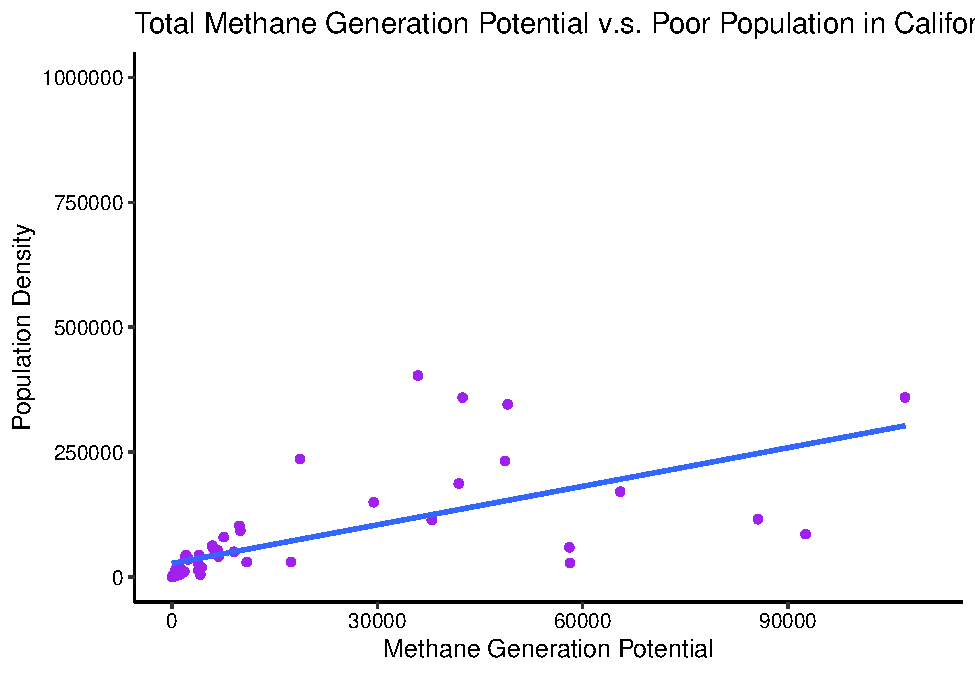
\includegraphics{FDR_Final_files/figure-latex/unnamed-chunk-8-1.pdf}
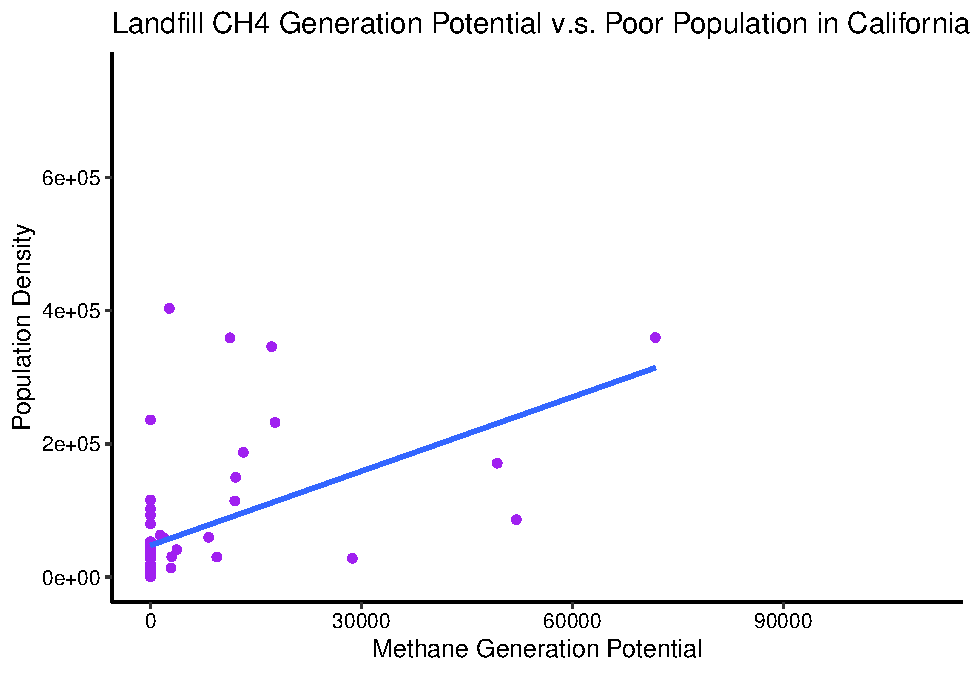
\includegraphics{FDR_Final_files/figure-latex/unnamed-chunk-8-2.pdf}
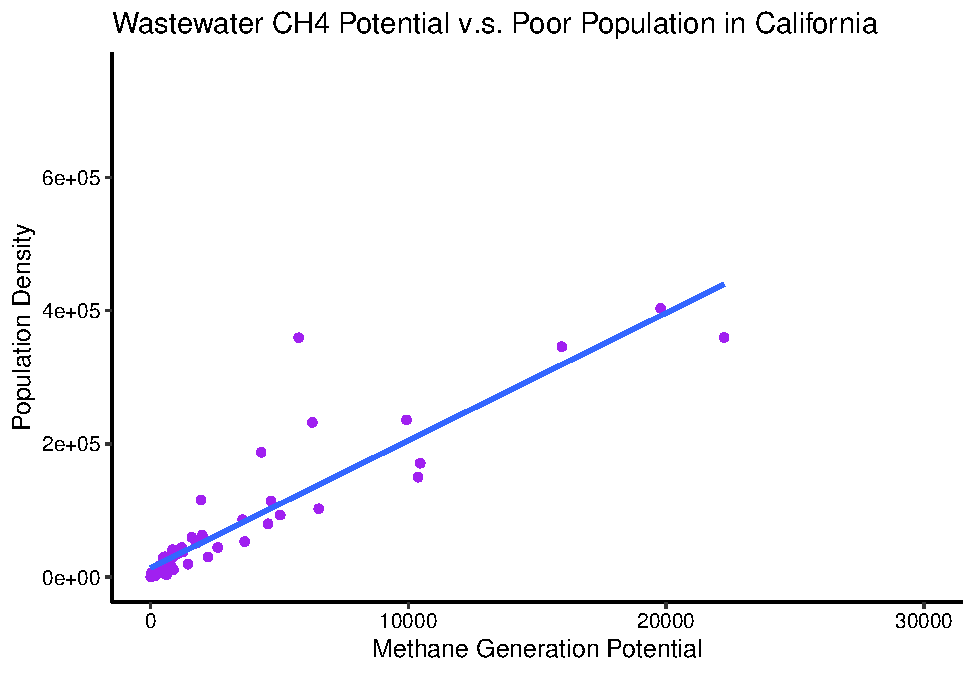
\includegraphics{FDR_Final_files/figure-latex/unnamed-chunk-8-3.pdf}
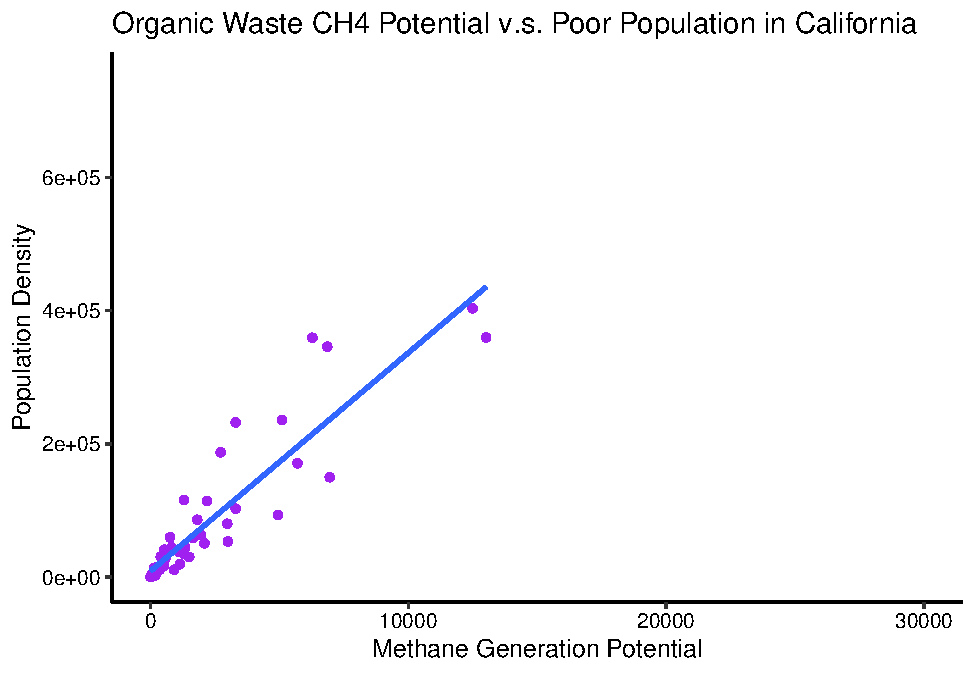
\includegraphics{FDR_Final_files/figure-latex/unnamed-chunk-8-4.pdf}
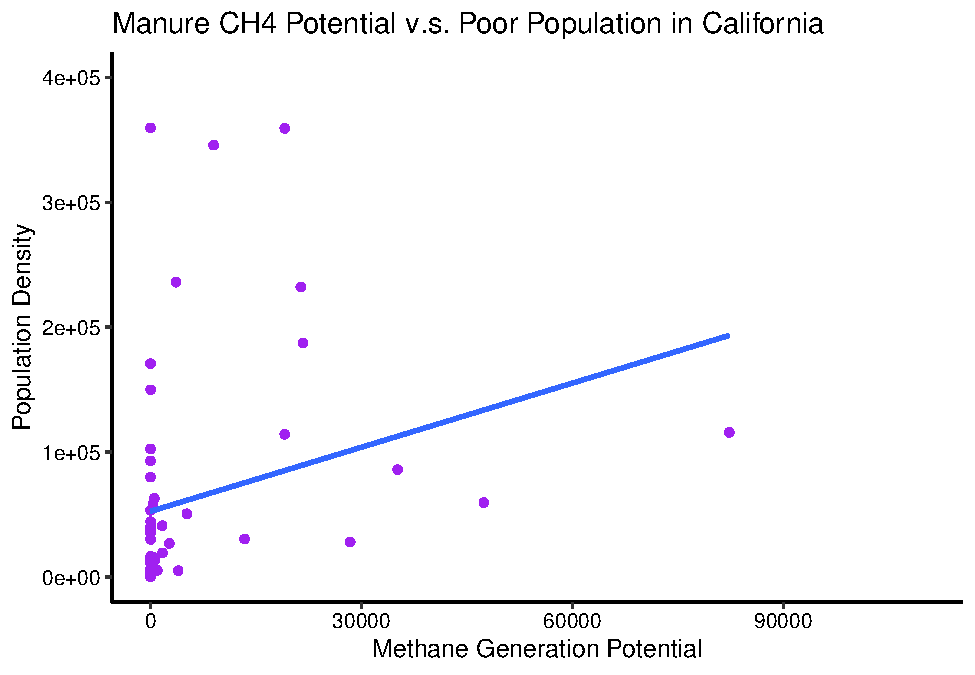
\includegraphics{FDR_Final_files/figure-latex/unnamed-chunk-8-5.pdf}

\newpage

\hypertarget{conclusion}{%
\section{Conclusion}\label{conclusion}}

The null hypothesis to our research question is that there is no
correlation between population density and biogas generation potential.
We ran a correlation test to test the strength and direction between
California population and the total biogas generation potential. We also
ran a simple linear regression model to investigate whether these two
variables involves a linear relationship. By looking at the residual
plots, we can tell that the regression model fits our data but has
outliers that disrupt the model accuracy. The p-value is 4.22e-15,
indicating that the result is statistically significant. The multiple
R-squared is 0.67, meaning that the independent variables can expalin
67\% of the variations in biogas generation potential. Therefore, we are
confident in rejecting the null hypothesis. Now we can say the total
biogas generation potential in california does have a linear
relationship with the population density. However, we still want to know
how and what different sources is correlated with population.
Subsequently, we ran the same test for each individual biogas sources.
Based on the results from running correlation test and linear regression
model for each of the biogas generation sources: Organic waste, Animal
manure, Wastewater, and Landfill. We found out the the organic waste and
wastewater contributes to the highest correlation to the population
density, while Animal manure and landfill are less correlated.

Overall, the analysis conducted show that biogas generation potential
across counties in California is positively correlated with the
population density. This implies that the higher the population in a
specific area, the higher the biogas generation potential. However, the
analysis also recognises that generation potential and correlation with
population density varies according to the biomass source across
counties. As such, results show that animal based methane appeared to be
less correlated with population. Assumptions that best explain this
result are that more animals will contribute to animal-based biomass and
that human habitation is often less where animal population is dense.
Results of our analysis also show that the potential of landfill-based
biogas was not limited to densely or sparsely populated areas, while
organic waste and waste water represented the most significant sources
of biogas generation potential across California.

Future analysis can focus on improving the model presented in this
report by eliminating some outliers and using more recent datasets. This
study made use of older data sets because those were the ones most
recently made available on open and credible data portals. Other areas
of future analysis include exploring the level and process of
utilization of California's biogas generation potential, as well as how
utilization can be scaled. For example, the potential of leveraging the
biogas generation potential by enabling counties with lower generation
potentials to tap into the resources for those with higher
generation.This also includes scoping the potential to utilize biogas
energy for base load power or peaking, using various analyses including
a cost-benefit analysis.

\newpage

\hypertarget{references}{%
\section{References}\label{references}}

\textless add references here if relevant, otherwise delete this
section\textgreater{}

\end{document}
